\documentclass[conference]{IEEEtran}
% Some Computer Society conferences also require the compsoc mode option,
% but others use the standard conference format.
%
% If IEEEtran.cls has not been installed into the LaTeX system files,
% manually specify the path to it like:
% \documentclass[conference]{../sty/IEEEtran}


\usepackage{color}
\usepackage{graphicx}
%\usepackage[top=0.5in,bottom=0.5in]{geometry}
% Some very useful LaTeX packages include:
% (uncomment the ones you want to load)


% *** MISC UTILITY PACKAGES ***
%
%\usepackage{ifpdf}
% Heiko Oberdiek's ifpdf.sty is very useful if you need conditional
% compilation based on whether the output is pdf or dvi.
% usage:
% \ifpdf
%   % pdf code
% \else
%   % dvi code
% \fi
% The latest version of ifpdf.sty can be obtained from:
% http://www.ctan.org/pkg/ifpdf
% Also, note that IEEEtran.cls V1.7 and later provides a builtin
% \ifCLASSINFOpdf conditional that works the same way.
% When switching from latex to pdflatex and vice-versa, the compiler may
% have to be run twice to clear warning/error messages.






% *** CITATION PACKAGES ***
%
%\usepackage{cite}
% cite.sty was written by Donald Arseneau
% V1.6 and later of IEEEtran pre-defines the format of the cite.sty package
% \cite{} output to follow that of the IEEE. Loading the cite package will
% result in citation numbers being automatically sorted and properly
% "compressed/ranged". e.g., [1], [9], [2], [7], [5], [6] without using
% cite.sty will become [1], [2], [5]--[7], [9] using cite.sty. cite.sty's
% \cite will automatically add leading space, if needed. Use cite.sty's
% noadjust option (cite.sty V3.8 and later) if you want to turn this off
% such as if a citation ever needs to be enclosed in parenthesis.
% cite.sty is already installed on most LaTeX systems. Be sure and use
% version 5.0 (2009-03-20) and later if using hyperref.sty.
% The latest version can be obtained at:
% http://www.ctan.org/pkg/cite
% The documentation is contained in the cite.sty file itself.






% *** GRAPHICS RELATED PACKAGES ***
%
\ifCLASSINFOpdf
  % \usepackage[pdftex]{graphicx}
  % declare the path(s) where your graphic files are
  % \graphicspath{{../pdf/}{../jpeg/}}
  % and their extensions so you won't have to specify these with
  % every instance of \includegraphics
  % \DeclareGraphicsExtensions{.pdf,.jpeg,.png}
\else
  % or other class option (dvipsone, dvipdf, if not using dvips). graphicx
  % will default to the driver specified in the system graphics.cfg if no
  % driver is specified.
  % \usepackage[dvips]{graphicx}
  % declare the path(s) where your graphic files are
  % \graphicspath{{../eps/}}
  % and their extensions so you won't have to specify these with
  % every instance of \includegraphics
  % \DeclareGraphicsExtensions{.eps}
\fi
% graphicx was written by David Carlisle and Sebastian Rahtz. It is
% required if you want graphics, photos, etc. graphicx.sty is already
% installed on most LaTeX systems. The latest version and documentation
% can be obtained at: 
% http://www.ctan.org/pkg/graphicx
% Another good source of documentation is "Using Imported Graphics in
% LaTeX2e" by Keith Reckdahl which can be found at:
% http://www.ctan.org/pkg/epslatex
%
% latex, and pdflatex in dvi mode, support graphics in encapsulated
% postscript (.eps) format. pdflatex in pdf mode supports graphics
% in .pdf, .jpeg, .png and .mps (metapost) formats. Users should ensure
% that all non-photo figures use a vector format (.eps, .pdf, .mps) and
% not a bitmapped formats (.jpeg, .png). The IEEE frowns on bitmapped formats
% which can result in "jaggedy"/blurry rendering of lines and letters as
% well as large increases in file sizes.
%
% You can find documentation about the pdfTeX application at:
% http://www.tug.org/applications/pdftex





% *** MATH PACKAGES ***
%
%\usepackage{amsmath}
% A popular package from the American Mathematical Society that provides
% many useful and powerful commands for dealing with mathematics.
%
% Note that the amsmath package sets \interdisplaylinepenalty to 10000
% thus preventing page breaks from occurring within multiline equations. Use:
%\interdisplaylinepenalty=2500
% after loading amsmath to restore such page breaks as IEEEtran.cls normally
% does. amsmath.sty is already installed on most LaTeX systems. The latest
% version and documentation can be obtained at:
% http://www.ctan.org/pkg/amsmath





% *** SPECIALIZED LIST PACKAGES ***
%
%\usepackage{algorithmic}
% algorithmic.sty was written by Peter Williams and Rogerio Brito.
% This package provides an algorithmic environment fo describing algorithms.
% You can use the algorithmic environment in-text or within a figure
% environment to provide for a floating algorithm. Do NOT use the algorithm
% floating environment provided by algorithm.sty (by the same authors) or
% algorithm2e.sty (by Christophe Fiorio) as the IEEE does not use dedicated
% algorithm float types and packages that provide these will not provide
% correct IEEE style captions. The latest version and documentation of
% algorithmic.sty can be obtained at:
% http://www.ctan.org/pkg/algorithms
% Also of interest may be the (relatively newer and more customizable)
% algorithmicx.sty package by Szasz Janos:
% http://www.ctan.org/pkg/algorithmicx




% *** ALIGNMENT PACKAGES ***
%
%\usepackage{array}
% Frank Mittelbach's and David Carlisle's array.sty patches and improves
% the standard LaTeX2e array and tabular environments to provide better
% appearance and additional user controls. As the default LaTeX2e table
% generation code is lacking to the point of almost being broken with
% respect to the quality of the end results, all users are strongly
% advised to use an enhanced (at the very least that provided by array.sty)
% set of table tools. array.sty is already installed on most systems. The
% latest version and documentation can be obtained at:
% http://www.ctan.org/pkg/array


% IEEEtran contains the IEEEeqnarray family of commands that can be used to
% generate multiline equations as well as matrices, tables, etc., of high
% quality.




% *** SUBFIGURE PACKAGES ***
%\ifCLASSOPTIONcompsoc
%  \usepackage[caption=false,font=normalsize,labelfont=sf,textfont=sf]{subfig}
%\else
%  \usepackage[caption=false,font=footnotesize]{subfig}
%\fi
% subfig.sty, written by Steven Douglas Cochran, is the modern replacement
% for subfigure.sty, the latter of which is no longer maintained and is
% incompatible with some LaTeX packages including fixltx2e. However,
% subfig.sty requires and automatically loads Axel Sommerfeldt's caption.sty
% which will override IEEEtran.cls' handling of captions and this will result
% in non-IEEE style figure/table captions. To prevent this problem, be sure
% and invoke subfig.sty's "caption=false" package option (available since
% subfig.sty version 1.3, 2005/06/28) as this is will preserve IEEEtran.cls
% handling of captions.
% Note that the Computer Society format requires a larger sans serif font
% than the serif footnote size font used in traditional IEEE formatting
% and thus the need to invoke different subfig.sty package options depending
% on whether compsoc mode has been enabled.
%
% The latest version and documentation of subfig.sty can be obtained at:
% http://www.ctan.org/pkg/subfig




% *** FLOAT PACKAGES ***
%
%\usepackage{fixltx2e}
% fixltx2e, the successor to the earlier fix2col.sty, was written by
% Frank Mittelbach and David Carlisle. This package corrects a few problems
% in the LaTeX2e kernel, the most notable of which is that in current
% LaTeX2e releases, the ordering of single and double column floats is not
% guaranteed to be preserved. Thus, an unpatched LaTeX2e can allow a
% single column figure to be placed prior to an earlier double column
% figure.
% Be aware that LaTeX2e kernels dated 2015 and later have fixltx2e.sty's
% corrections already built into the system in which case a warning will
% be issued if an attempt is made to load fixltx2e.sty as it is no longer
% needed.
% The latest version and documentation can be found at:
% http://www.ctan.org/pkg/fixltx2e


%\usepackage{stfloats}
% stfloats.sty was written by Sigitas Tolusis. This package gives LaTeX2e
% the ability to do double column floats at the bottom of the page as well
% as the top. (e.g., "\begin{figure*}[!b]" is not normally possible in
% LaTeX2e). It also provides a command:
%\fnbelowfloat
% to enable the placement of footnotes below bottom floats (the standard
% LaTeX2e kernel puts them above bottom floats). This is an invasive package
% which rewrites many portions of the LaTeX2e float routines. It may not work
% with other packages that modify the LaTeX2e float routines. The latest
% version and documentation can be obtained at:
% http://www.ctan.org/pkg/stfloats
% Do not use the stfloats baselinefloat ability as the IEEE does not allow
% \baselineskip to stretch. Authors submitting work to the IEEE should note
% that the IEEE rarely uses double column equations and that authors should try
% to avoid such use. Do not be tempted to use the cuted.sty or midfloat.sty
% packages (also by Sigitas Tolusis) as the IEEE does not format its papers in
% such ways.
% Do not attempt to use stfloats with fixltx2e as they are incompatible.
% Instead, use Morten Hogholm'a dblfloatfix which combines the features
% of both fixltx2e and stfloats:
%
% \usepackage{dblfloatfix}
% The latest version can be found at:
% http://www.ctan.org/pkg/dblfloatfix




% *** PDF, URL AND HYPERLINK PACKAGES ***
%
%\usepackage{url}
% url.sty was written by Donald Arseneau. It provides better support for
% handling and breaking URLs. url.sty is already installed on most LaTeX
% systems. The latest version and documentation can be obtained at:
% http://www.ctan.org/pkg/url
% Basically, \url{my_url_here}.




% *** Do not adjust lengths that control margins, column widths, etc. ***
% *** Do not use packages that alter fonts (such as pslatex).         ***
% There should be no need to do such things with IEEEtran.cls V1.6 and later.
% (Unless specifically asked to do so by the journal or conference you plan
% to submit to, of course. )


% correct bad hyphenation here
\hyphenation{op-tical net-works semi-conduc-tor}


\begin{document}
%
% paper title
% Titles are generally capitalized except for words such as a, an, and, as,
% at, but, by, for, in, nor, of, on, or, the, to and up, which are usually
% not capitalized unless they are the first or last word of the title.
% Linebreaks \\ can be used within to get better formatting as desired.
% Do not put math or special symbols in the title.
\title{Experimental Evaluation of Co-design of Computation and Control for Autonomous Navigation \vspace{-0.3cm}}


% author names and affiliations
% use a multiple column layout for up to three different
% affiliations
%\author{\IEEEauthorblockN{Michael Shell}
%\IEEEauthorblockA{School of Electrical and\\Computer Engineering\\
%Georgia Institute of Technology\\
%Atlanta, Georgia 30332--0250\\
%Email: http://www.michaelshell.org/contact.html}
%\and
%\IEEEauthorblockN{Homer Simpson}
%\IEEEauthorblockA{Twentieth Century Fox\\
%Springfield, USA\\
%Email: homer@thesimpsons.com}
%\and
%\IEEEauthorblockN{James Kirk\\ and Montgomery Scott}
%\IEEEauthorblockA{Starfleet Academy\\
%San Francisco, California 96678--2391\\
%Telephone: (800) 555--1212\\
%Fax: (888) 555--1212}}

% conference papers do not typically use \thanks and this command
% is locked out in conference mode. If really needed, such as for
% the acknowledgment of grants, issue a \IEEEoverridecommandlockouts
% after \documentclass

% for over three affiliations, or if they all won't fit within the width
% of the page, use this alternative format:
% 

\author{
\IEEEauthorblockN{Nischal K. N., Paritosh Kelkar, Yash Vardhan Pant, Houssam Abbas, \\
	 Joseph Devietti, Rahul Mangharam}
\IEEEauthorblockA{The Departments of Electrical and Systems Engineering and Computer and Information Sciences, \\ University of Pennsylvania, Philadelphia, U.S.A.}
\vspace{-0.9cm}
%Atlanta, Georgia 30332--0250\\ Email: see http://www.michaelshell.org/contact.html}
%\IEEEauthorblockA{\IEEEauthorrefmark{2}Twentieth Century Fox, Springfield, USA\\
%Email: homer@thesimpsons.com}
%\IEEEauthorblockA{\IEEEauthorrefmark{3}Starfleet Academy, San Francisco, California 96678-2391\\
%Telephone: (800) 555--1212, Fax: (888) 555--1212}
%\IEEEauthorblockA{\IEEEauthorrefmark{4}Tyrell Inc., 123 Replicant Street, Los Angeles, California 90210--4321}}
}



% use for special paper notices
%\IEEEspecialpapernotice{(Invited Paper)}




% make the title area
\maketitle

% As a general rule, do not put math, special symbols or citations
% in the abstract

\begin{abstract}
The research on autonomous cars has been around for a while. A lot of algorithms are readily available for navigation at low update rates, however none of them have been targeted at high speeds. This work aims to execute similar tasks at high speeds while maintaining most optimized race lines and avoiding dynamic obstacles using minimalistic hardware. The concept is demonstrated on a 1/10th scale RC race car.
\vspace{0.05cm}
\end{abstract}

% no keywords




% For peer review papers, you can put extra information on the cover
% page as needed:
% \ifCLASSOPTIONpeerreview
% \begin{center} \bfseries EDICS Category: 3-BBND \end{center}
% \fi
%
% For peerreview papers, this IEEEtran command inserts a page break and
% creates the second title. It will be ignored for other modes.
\IEEEpeerreviewmaketitle

The platform used is a Traxxas 74076 Rally car which can achieve speeds of 40mph+ powered by a Velineon 3500 Brushless Motor and a 7 cell NiMH battery. Low Center of Gravity and 4WD enable precise control of position and velocity. The sensor system on board consists of a Firefly MV 0.3 MP USB camera, Hokuyu URG-04lx Lidar and an Razor IMU. The camera is coupled with a wide angle lens mounted on the front with update rates of upto 60Hz. Lidar is mounted at the rear and provides with a 2D laser scan at a rate of 10Hz. The Razor IMU has 9DOF (3 axis gyro, 3 axis accelerometer and 3 axis magnetometer) with an update rate of 50Hz. 

The processor on board is a Quad-Core ARM Cortex-A15 Nvidea Tegra K1 supplemented by a 192 core GPU and 2GB of RAM. The processor operates over a range of 204MHz to 2.3GHz based on the demand for accuracy needed. The GPU has a frequency range of 72MHz to 852MHz. The processor handles most of the control algorithms whereas the GPU handles the computer vision algorithms. 

The software structure of the car can be broken down into mapping, localization, path planning and control. Here we are using ORB SLAM\cite{ORB} for mapping through the front mounted wide angle camera. It performs a monocular SLAM in real time and generates a 3D map of the environment with large loop closures. The pose and localization is estimated through ORB SLAM supplemented by an IMU. The Ethzasl multi sensor fusion (MSF)\cite{MSF} framework (based on the EKF) is used for fusing localization data from the camera and IMU readings. A state-lattice based path planner generatates multiple trajectories, taking in information from the state estimation for localization and the Lidar for obstacle detection to form a cost map. The best (optimal, and safe) trajectory is selected to be followed. Trajectory tracking is done by a feedback based controller. The path planner also runs at 10Hz.

In order to operate at high speeds, computationally heavy tasks in the toolchain, namely ORB SLAM and the path planner need execute faster than is possible with out-of-the box implementations on the current hardware. In order to overcome this limitation we propose contract based co-design for the perception and control as detailed in \cite{RTSS15}. %The focus of demo and poster following this write-up will be on the expertimental evaluation of contract based execution of the perception/estimaion and path planning impacts the control performance (with and without a co-designed controller). 
It is worth noting that in out-of-the box implementations, the planner, perception (ORB SLAM), state estimation (MSF), and the control algorithm all compete for the same execution resources, the CPU. In our experimental evaluation of perception based corridor navigation with non-linear feedback control \cite{complex15}, we show how scheduling computation tasks on the CPU or the GPU and varying the computation frequency of the CPU/GPU can result in either faster and more power-hungry or slower but more power efficient execution. A feedback based supervisory algorithm decides the resource allocation and CPU/GPU frequencies in order to be efficient with computation power but also provide fast enough feedback updates for the controller. Ongoing work focuses on applying co-design for the entire percpetion, estimation, planning and control toolchain.


%\textcolor{red}{Have to write about path planner algorithm and control algorithm.} \\


%To train the controller on various knobs available for it to optimize based on the circumstances, a offline profiling of performance vs power is performed. For a pre recorded data sequence (camera and IMU), the performance of the car is compared with the ground truth obtained through an Vicon motion capture system at various GPU and CPU clock speeds along with the other parameters that can be tuned at various stages of the algorithm. Fig.  \\

%\textcolor{red}{What do we demo???? Im not sure}


\begin{figure}[bt]
\centering
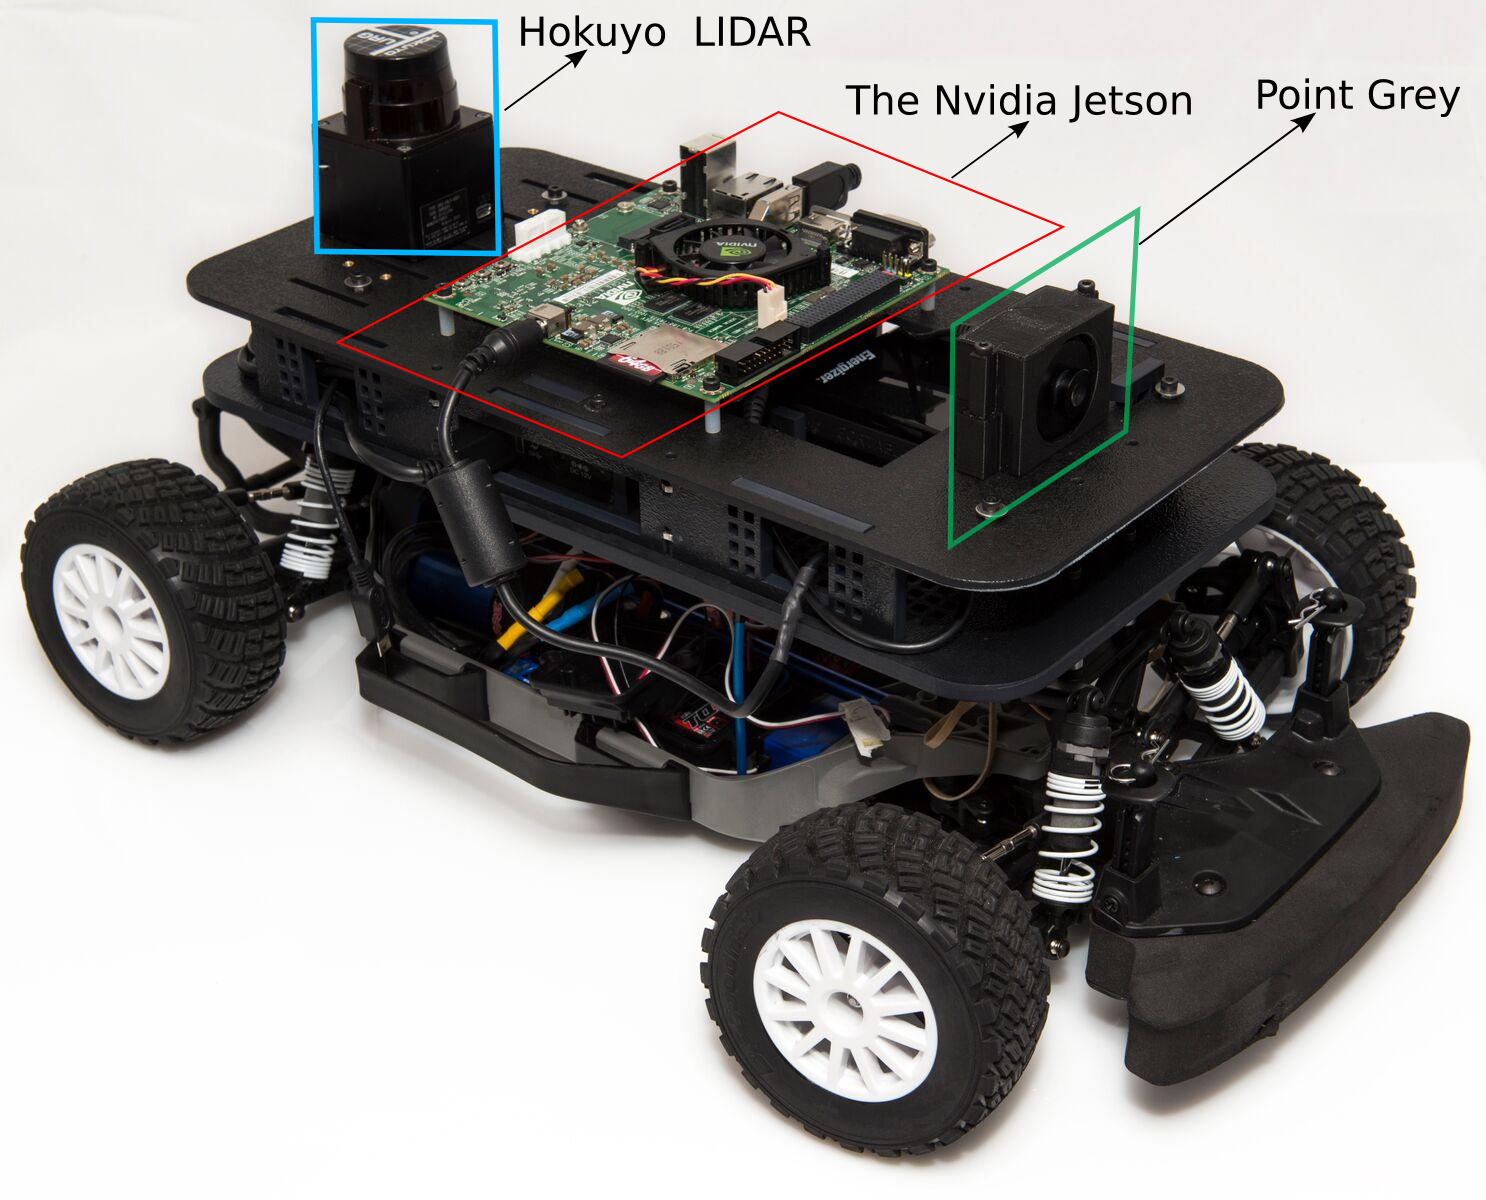
\includegraphics[scale=0.15]{car_labeled.png}
\caption{Race car platform with various sensors onboard}
\vspace{-0.7cm}
\end{figure}

%\section*{Acknowledgment}

%The authors would like to thank...





% trigger a \newpage just before the given reference
% number - used to balance the columns on the last page
% adjust value as needed - may need to be readjusted if
% the document is modified later
%\IEEEtriggeratref{8}
% The "triggered" command can be changed if desired:
%\IEEEtriggercmd{\enlargethispage{-5in}}

% references section

% can use a bibliography generated by BibTeX as a .bbl file
% BibTeX documentation can be easily obtained at:
% http://mirror.ctan.org/biblio/bibtex/contrib/doc/
% The IEEEtran BibTeX style support page is at:
% http://www.michaelshell.org/tex/ieeetran/bibtex/
%\bibliographystyle{IEEEtran}
% argument is your BibTeX string definitions and bibliography database(s)
%\bibliography{IEEEabrv,../bib/paper}
%
% <OR> manually copy in the resultant .bbl file
% set second argument of \begin to the number of references
% (used to reserve space for the reference number labels box)

\begin{thebibliography}{1}
\bibitem{ORB}
R. Mur-Artal, J. M. M. Montiel and J. D. Tard\'{o}s, \emph{ORB-SLAM: A Versatile and Accurate Monocular SLAM System}, IEEE Transactions on Robotics, vol. 31, no. 5, pp. 1147-1163, 2015.
\bibitem{MSF}
S. Lynen and M. Achtelik and S. Weiss and M. Chli and R. Siegwart, \emph{A Robust and Modular Multi-Sensor Fusion Approach Applied to MAV Navigation}, Proc. of the IEEE/RSJ Conference on Intelligent Robots and Systems (IROS), 2013.
\bibitem{RTSS15}
	Y.V. Pant and H. Abbas and K. Mohta and T.X. Nghiem and J. Devietti and R. Mangharam, \emph{Co-design of Anytime Computation and Robust Control}, to be published in Proc. of the IEEE Real Time Systems Symposium (RTSS), 2015.	
\bibitem{complex15}
	Y.V. Pant and H. Abbas and Nishcal K.N. and P. Kelkar and D. Kumar and J. Devietti and R. Mangharam \emph{Power-efficient algorithms for autonomous navigation}, to be published in the Proc. of the IEEE Intl. Conference on Complex Systems Engineering (ICCSE), 2015.
\end{thebibliography}




% that's all folks
\end{document}


